\chapter{
  The LHC and CMS Experiment
 }\label{ch_cms}

The physics analysis is carried out using \gls{CMS} experiment at
\gls{CERN} \gls{LHC} accelerator. This chapter provides overview of \gls{LHC}
and detail of CMS experiment and its sub-detectors for particle tracking
and calorimetry.

\section{
  The Large Hadron Collider
 }\label{ch_cms:lhc}

The \gls{LHC} is the largest accelerator located at
\gls{CERN} in Geneva, Switzerland.
The main \gls{LHC} ring is 27\km{} in circumference
and around 50 to 175\m{} underground.
The \gls{LHC} is built to collide protons at 14\TeV{} center-of-mass energy,
LHC delivered proton-proton collisions at 7 and 8\TeV{}
during run-1 (2010--2012), and at 13\TeV{} center-of-mass energy during
run-2 (2015--2018)
~\cite{Evans:2008}.

The Figure~\ref{fig:lhc} describes \gls{CERN} accelerator complex.
The protons are sourced by ionizing hydrogen atoms
and then fed into \gls{LINAC}.
The \gls{LINAC} accelerates the protons to 50\MeV{} and sent to the booster.
Then the booster increases energy of protons to 1.4\GeV{} and
feeds it to the \gls{PS} which further increases energy to 25\GeV{}
and starts bunching them together with bunches 25\nanoseconds{} apart.
Then the proton bunches are passed through \gls{SPS} which increases energy
to 450\GeV{} and finally sent to main \gls{LHC} clockwise and counterclockwise
rings where they are accelerated to final energy required which is 6.5\TeV{}
for both bunches going clockwise and counterclockwise
to obtain collisions at 13\TeV{} center-of-mass energy.

The proton-proton collisions occurs at four different location where two
general purpose detectors \gls{CMS} and \gls{ATLAS}, and
two specific purpose detector \gls{ALICE} and \gls{LHCb} are located.

\begin{figure}[!ht]
  \centering
  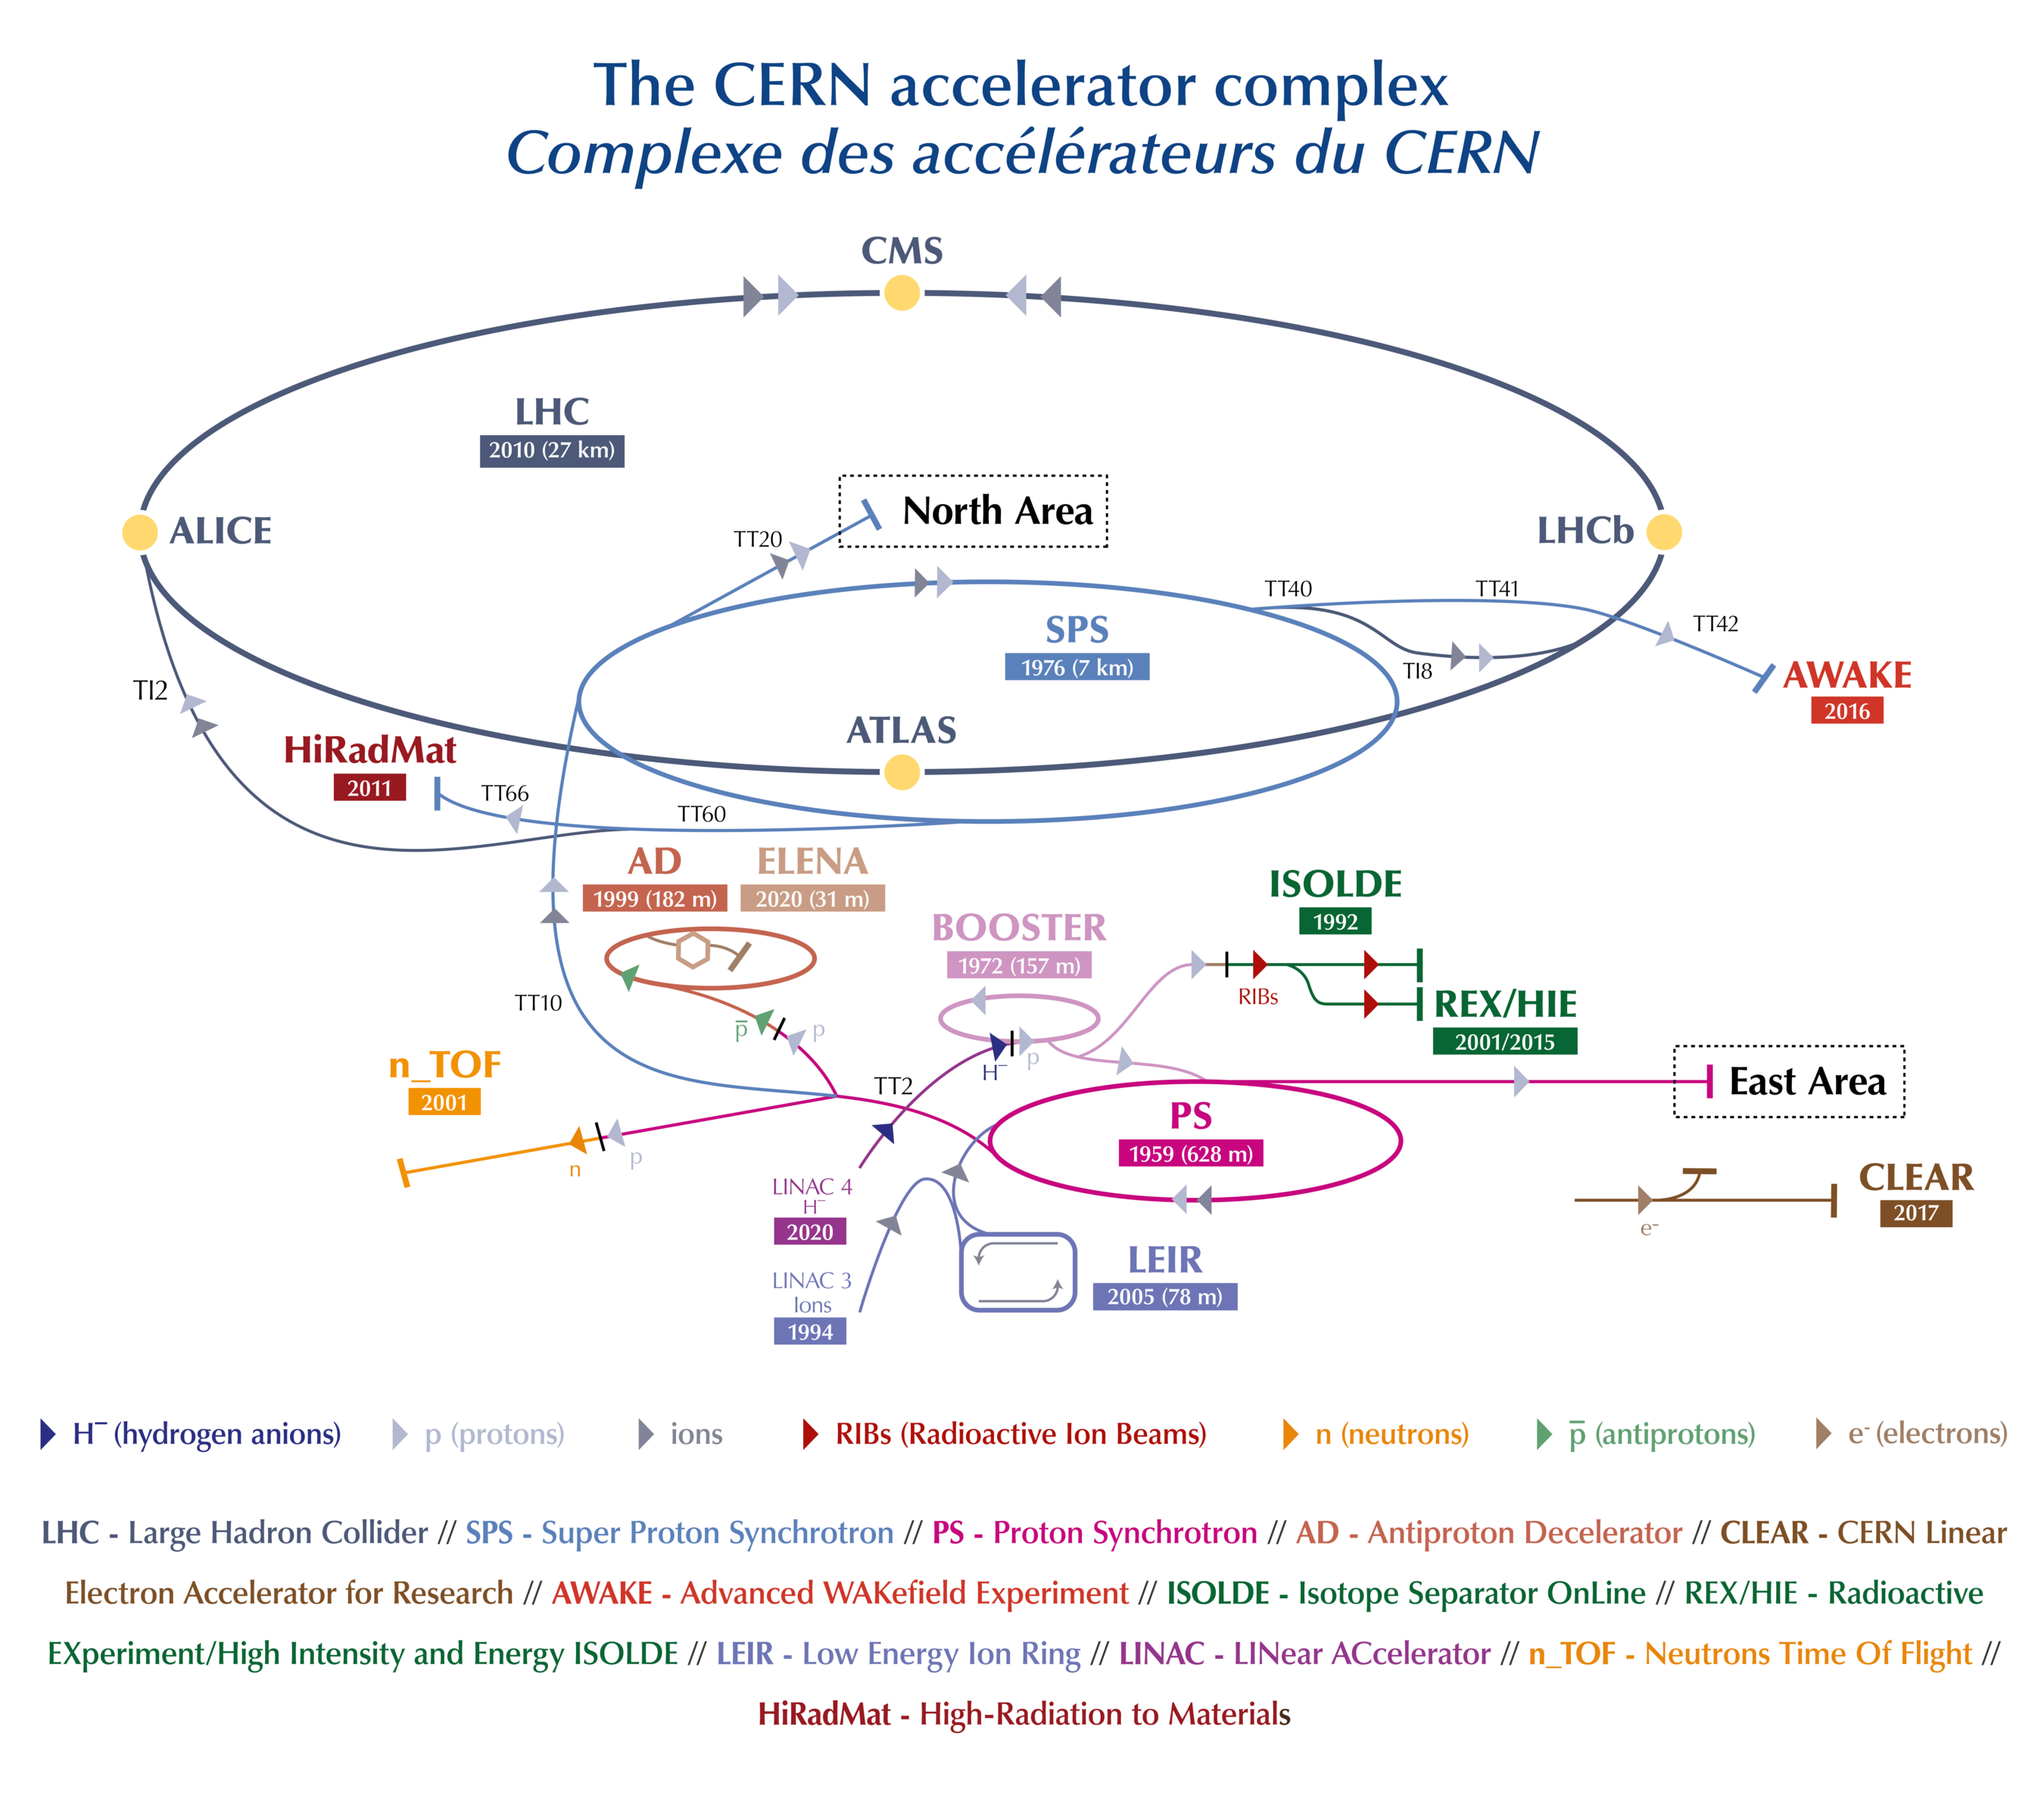
\includegraphics[width=0.98\textwidth]{figures/lhc-scheme.png}
  \caption[A schematic of the CERN accelerator complex]%
  {A schematic of the CERN accelerator complex~\cite{image-lhc-scheme}}%
  \label{fig:lhc}
\end{figure}

\subsection{
  Integrated Luminosity
}\label{ch_cms:cms-lumi}

The number of events generated in a collisions for a given process is
\begin{equation}
  N = L \sigma
\end{equation}
where \(\sigma \) is cross-section of the process
and \(L\) is the luminosity of the \gls{LHC}.

\begin{figure}[!ht]
  \centering
  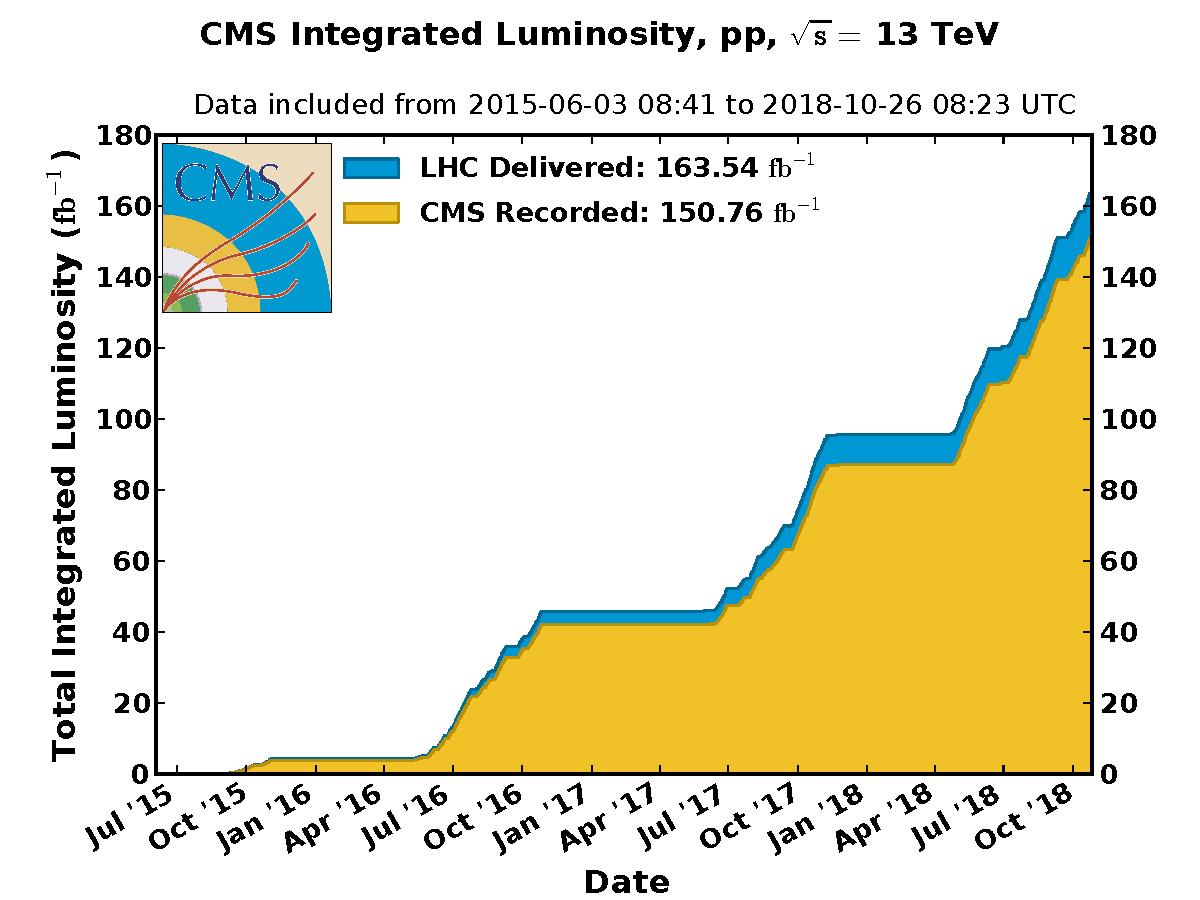
\includegraphics[width=0.5\textwidth]{figures/int_lumi_pp_run2.pdf}
  \caption[Cumulative delivered and recorded luminosity versus
    time for 2015--2018 proton-proton collisions]%
  {Cumulative delivered and recorded luminosity versus
    time for 2015--2018 proton-proton collisions~\cite{plot-cms-lumi}}%
  \label{fig:int-lumi}
\end{figure}

Cumulative luminosity delivered and recorded by \gls{CMS} during run-2 operation
in shown in Figure~\ref{fig:int-lumi}.
For run-2 standard physics analysis luminosity recorded during
2016--2018 is considered, and only runs certified as ``golden'' by \gls{CMS}
Luminosity \gls{POG} for analysis are used. The total luminosity for run-2
standard physics is 137.19\fbinv{}
and separately for years in Table~\ref{tab:years-lumi}
~\cite{CMS-PAS-LUM-17-001,CMS-PAS-LUM-17-004,CMS-PAS-LUM-18-002}.

\begin{table}[!ht]
  \centering
  \caption[Standard physics luminosity for run-2]%
  {Standard physics luminosity for run-2}
  \begin{tabular}{cccc}
    \toprule
    2016          & 2017          & 2018          & run-2          \\ \midrule
    35.92\fbinv{} & 41.53\fbinv{} & 59.74\fbinv{} & 137.19\fbinv{} \\
    \bottomrule
  \end{tabular}%
  \label{tab:years-lumi}
\end{table}

\section{
  The CMS Detector
 }\label{ch_cms:cms}

The \gls{CMS} detector is a general purpose detector.
A cutaway view of the detector is shown in Figure~\ref{fig:cms-cutaway}.
The detector is cylindrical with dimensions 21 meters long, and 15 meters
in diameter, and the whole detector weighs about 14000 tonnes.
The detector is built in slices with central region called ``barrel'',
and two closing end sides called ``endcap''.
A superconducting solenoid generates magnetic field of 3.8\Tesla{} inside
and 2\Tesla{} outside, and to contain the magnetic field outside of solenoid
and support structure of the detector massive steel yokes are used.

\begin{figure}[!ht]
  \centering
  \includegraphics[width=\textwidth]{figures/cms_cutway_ME4_2.pdf}
  \caption[The CMS detector cutaway view]%
  {The CMS detector cutaway view~\cite{image-cms-cutway}}%
  \label{fig:cms-cutaway}
\end{figure}

The slice view of \gls{CMS} in Figure~\ref{fig:cms-slice}
shows how different particles leave signature in \gls{CMS} detector.
Neutral particles such photons, neutrinos, and hadrons will leave no track
in \gls{ST}, and are identified by only energy deposited or missing energy.
Electrons are identified from the track in \gls{ST} and energy deposit
in \gls{ECAL}, hadrons are heavier and they pass through \gls{ECAL}
and deposit their energy completely in \gls{HCAL}, leaving only small fraction
of energy in \gls{ECAL}.
Since muons are \gls{MIP}, they pass through whole detector with very small
fraction of energy deposit in \gls{ECAL} and \gls{HCAL}.

This section describes the subsystems of \gls{CMS} detector.
For detailed technical description refer to~\cite{CMS-JINST-S08004}.

\begin{figure}[!ht]
  \centering
  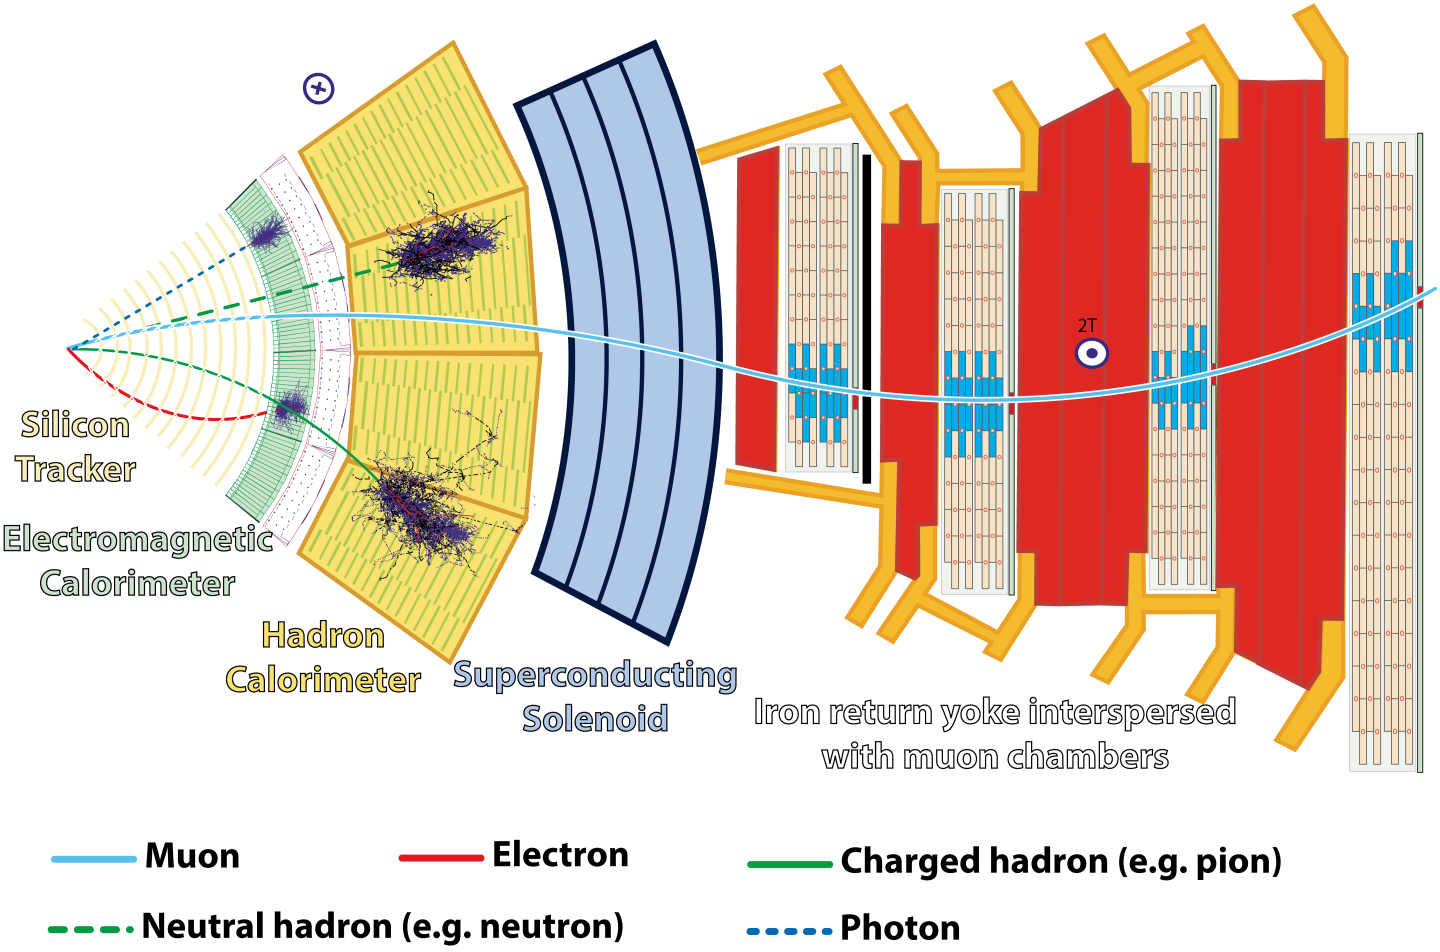
\includegraphics[width=\textwidth]{figures/cms_slice.png}
  \caption[The CMS detector slice view]%
  {The CMS detector slice view~\cite{image-cms-slice}}%
  \label{fig:cms-slice}
\end{figure}

\subsection{
  The CMS Coordinate System
}\label{ch_cms:cms-coordinate}

CMS uses \gls{IP} of collisions as origin to define right-handed
coordinate system. The \( z \)-axis is along the beamline,
the \( x \)-axis points toward the center of the \gls{LHC},
and the \( y \)-axis points upwards, toward Earth's surface.
The transverse plane \( x - y \) is used as to calculate
most commonly used quantities like transverse momentum \( p_{T} \)
and energy \( E_{T} \).

To describe the direction of particles leaving the \gls{IP},
azimuthal \( \phi \) and polar \( \theta \) angles are used.
\( \phi \) is measured around the beam axis,
and \( \theta \) is measured from the beam axis.
In collider physics, pseudorapidity \( \eta \) (Lorentz invariant) is used
to describe direction from beam pipe instead of \( \theta \) as,

\begin{equation}
  \eta = - \ln[\tan{\theta/2}]
\end{equation}

and sometimes in terms of rapidity \( y \) as,

\begin{equation}
  y = \frac{1}{2} \ln{\frac{E+p_{z}}{E-p_{z}}}
\end{equation}

Particles kinematics can be completely described in terms of
\( p_{T} \), \( \eta \), \( \phi \), and \( E_{T} \) or mass.
The distance between the two particles \( \Delta R \) in \( \eta - \phi \) plane
is described as,

\begin{equation}
  \Delta R = \sqrt{ {(\Delta \eta)}^{2} + {(\Delta \phi)}^{2} }
\end{equation}

\subsection{
  The Superconducting Magnet
}

The superconducting magnet is the main part of the \gls{CMS} detector, it is
12.5 meters long and 6.3 meters in diameter. The magnet is cooled to
4.5\,\text{K}\xspace and 20\,\text{kA}\xspace current flows through it to
generate 3.8\Tesla{} of magnetic field with stored energy of 2.6\,\text{GJ}\xspace.

The Figure~\ref{fig:cms-magnet} shows visible superconducting magnet
and iron yoke when part of \gls{CMS} detector was lowered in the underground
cavern during installation in 2007.

The key purpose of magnet is to determine the momentum and the sign of charged
particles by bending them. The momentum resolution of the particles will
decrease with increase in \(p_T \), with constant 3.8\Tesla{} magnetic field
inside and it has momentum resolution of \(\Delta p /p \approx 10 \% \), which
is enough to determine unambiguously the sign of muons with
momentum of \(\approx 1\TeV{}/c \).

\begin{figure}[!ht]
  \centering
  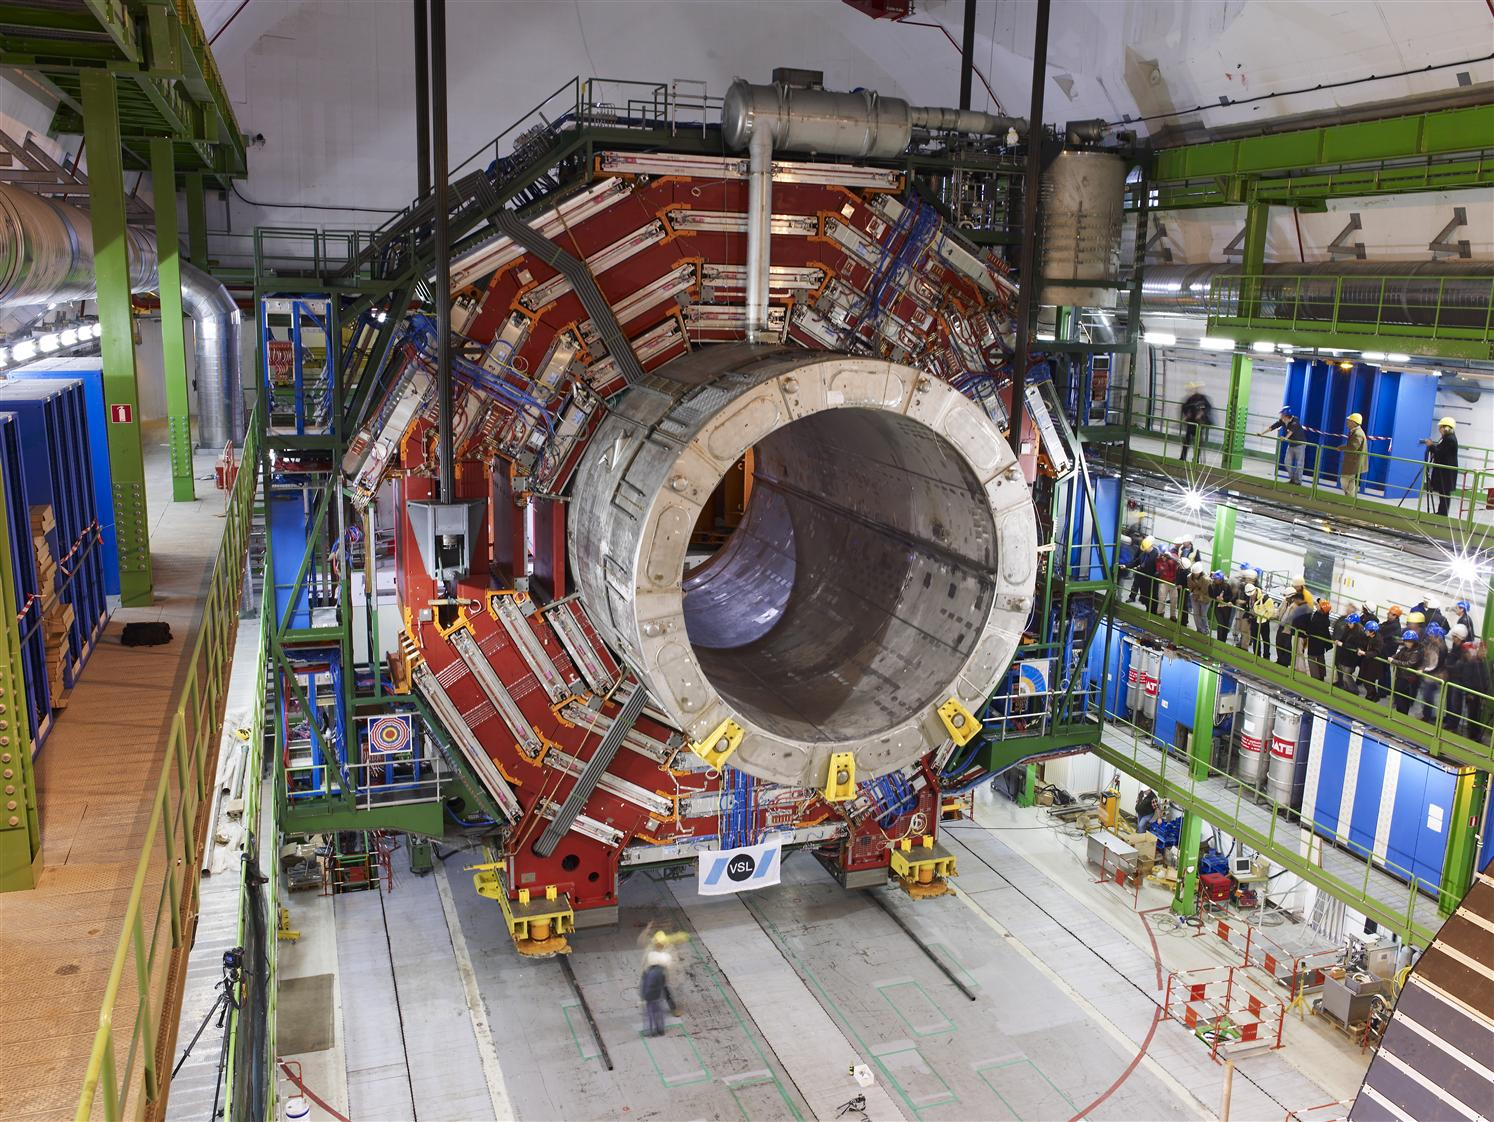
\includegraphics[width=0.75\textwidth]{figures/cms_magnet_lowered.jpg}
  \caption%
  [The picture of the CMS detector central part when lowered in underground
    cavern with superconducting magnet and iron
    yoke visible]%
  {The picture of the CMS detector central part when lowered in underground
    cavern with superconducting magnet and iron
    yoke visible~\cite{image-cms-magnet}.}%
  \label{fig:cms-magnet}
\end{figure}


\subsection{
  The Tracking System
}

The \gls{CMS} tracking system \gls{ST} is the innermost part of the detector, it
is made up of pixel and strip detectors. The main goal of \gls{ST} is to
reconstruct the tracks of the charged particles with high precision in high pileup
environment.

Silicon is most commonly used material for making tracking systems because of it's
semiconductor properties, and high radiation hardness which is essential for the
innermost detector. When a p-n junction is built on silicon substrate it creates
a depletion zone with no charge carriers at the junction, and whenever
a charged particle pass through the depletion zone it creates a electron-hole pair,
and under reverse bias this electron-hole generates electrical signal. The \gls{CMS}
tracking consists of about 124 million channels of such junctions in
pixel detector and 10 million in strip detector.

The pixel detector was upgraded in 2017 and the comparison of layers before
and after the upgrade is shown in Figure~\ref{fig:cms-pixel}. It is made up of
four barrel layers and three endcaps, with nearest barrel layer being 3\cm{}
away from beamline for precise measurement of \gls{IP}.
Because of the large number of pixel channels, the readout is done by \glspl{ASIC}.

\begin{figure}[!ht]
  \centering
  \begin{minipage}[c]{.62\textwidth}
    \includegraphics[trim={80pt 0 80pt 0},clip,width=\textwidth]%
    {figures/cms_pixel_phase1.pdf}
  \end{minipage}
  \begin{minipage}[c]{.35\textwidth}
    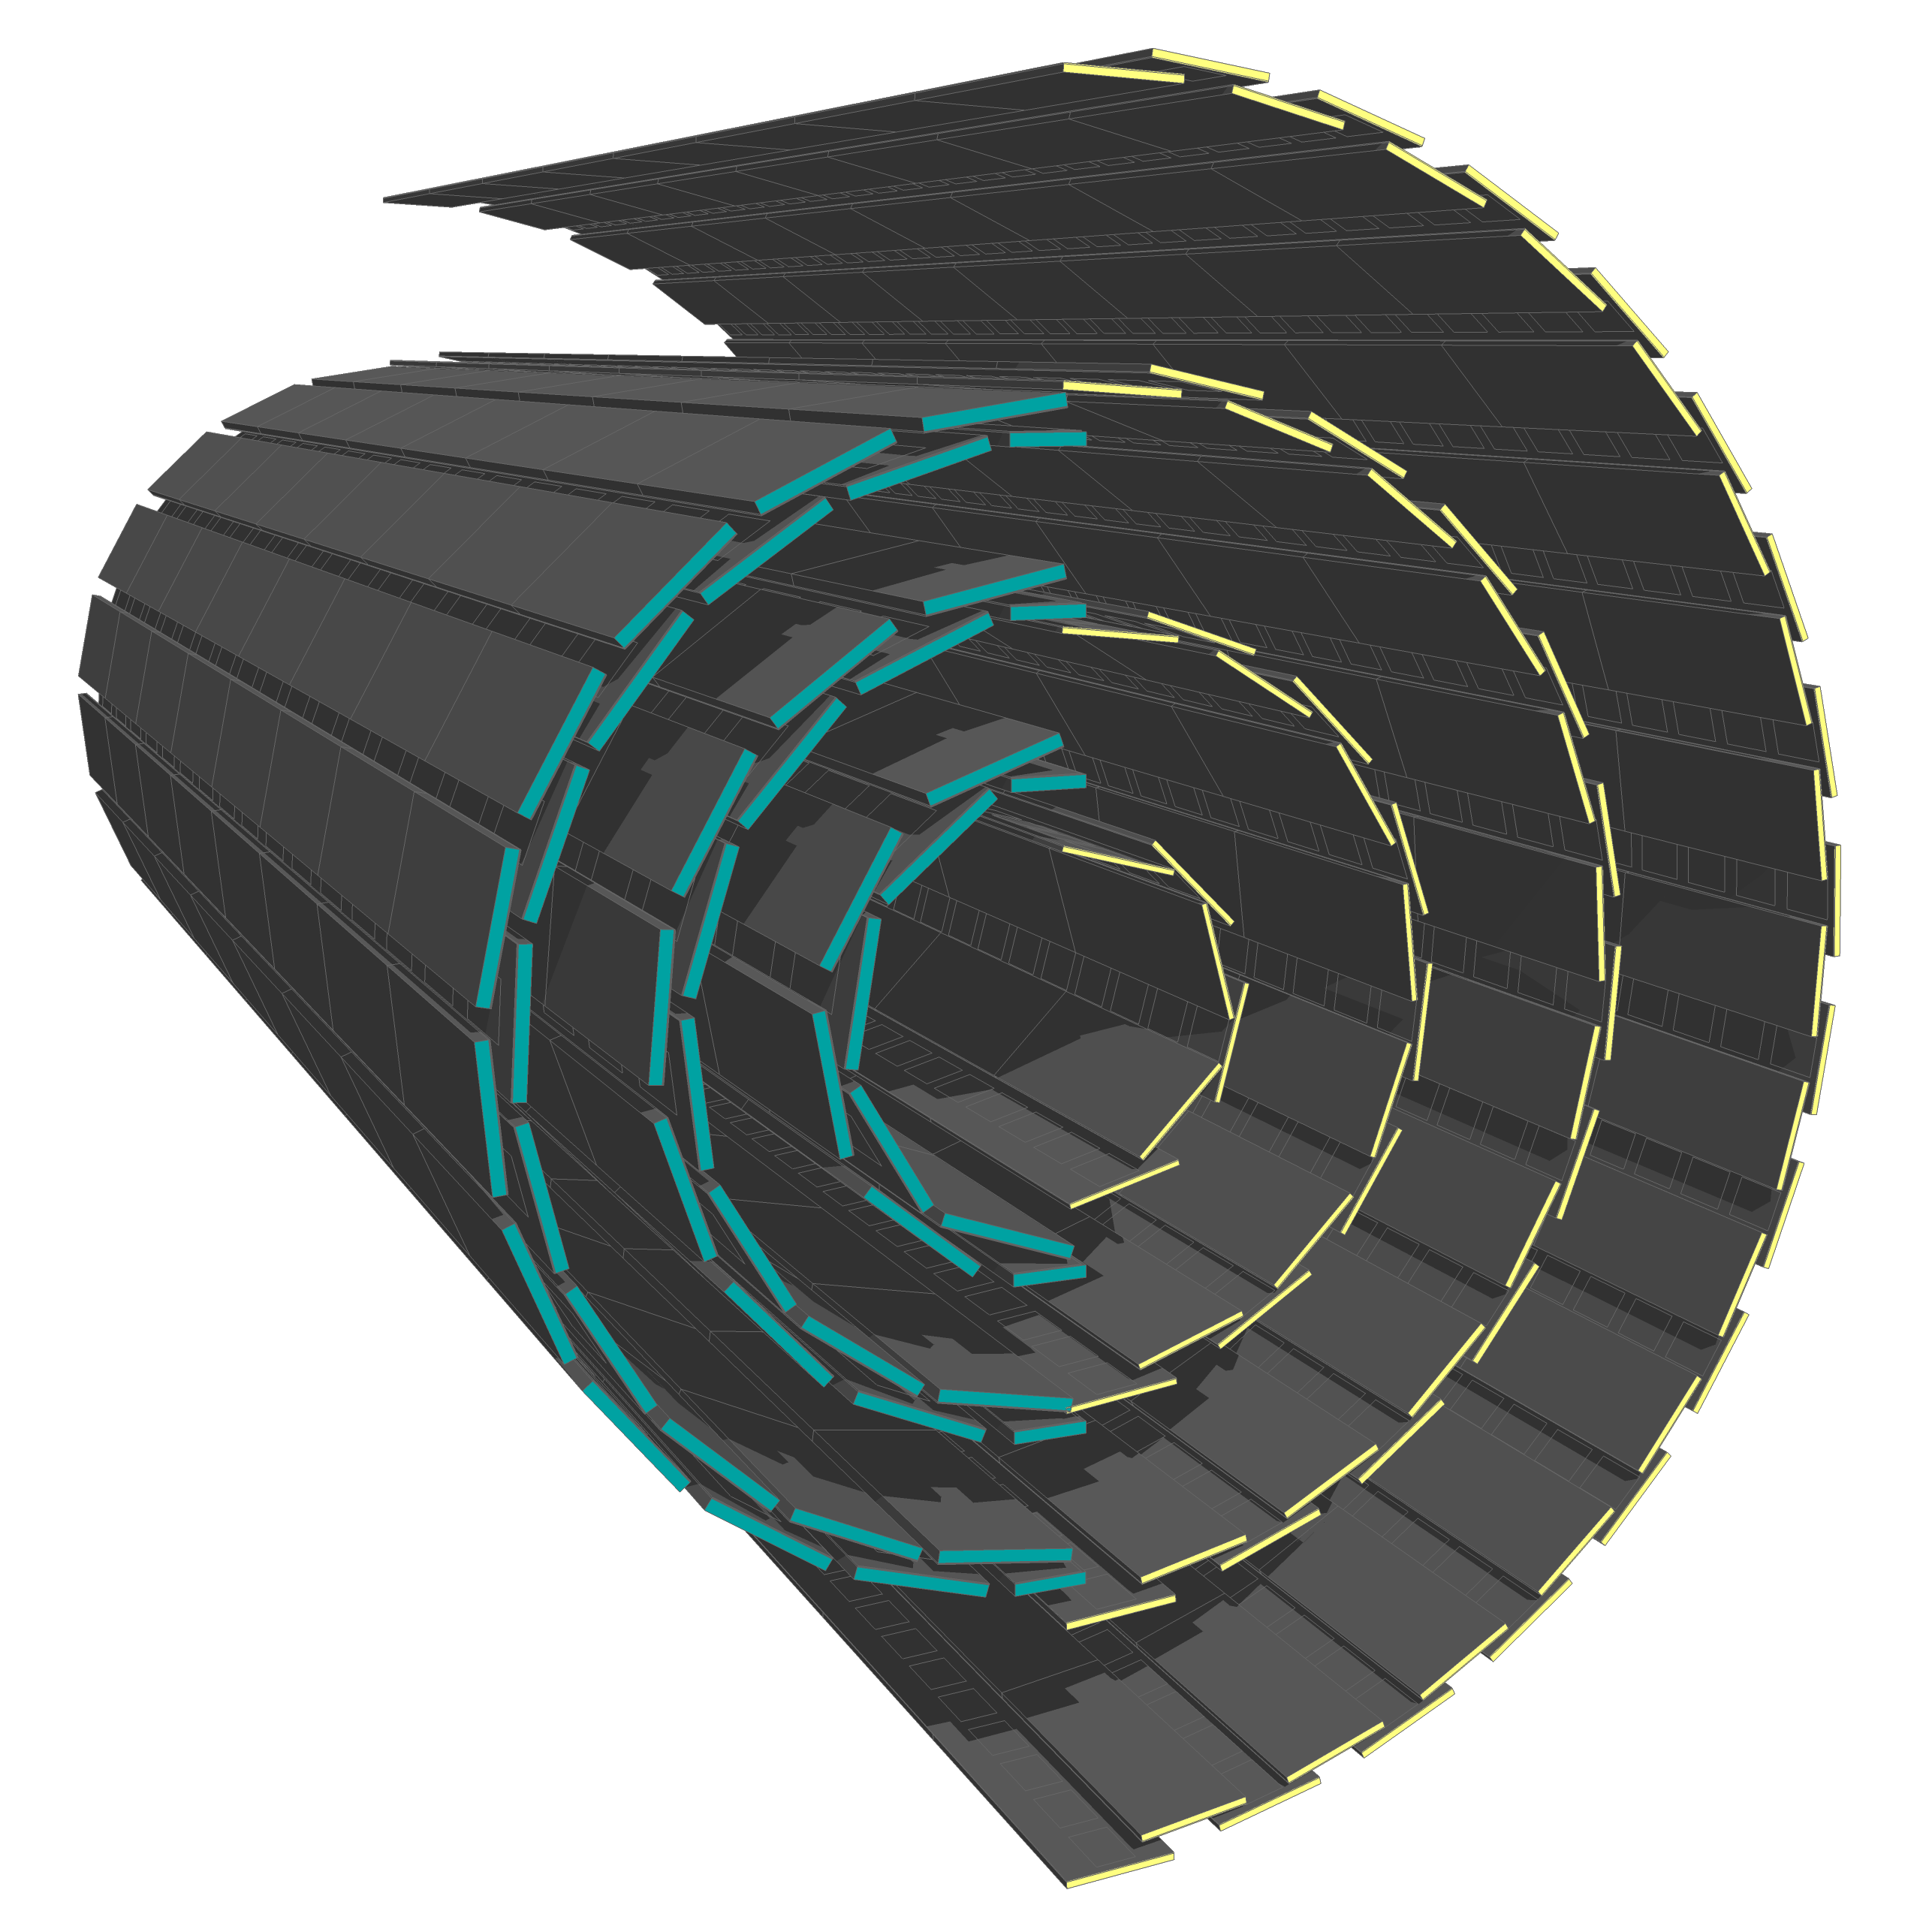
\includegraphics[width=\textwidth]{figures/cms_pixel_phase1_04.png}
  \end{minipage}
  \caption[The CMS pixel upgrade]%
  {The CMS pixel upgrade. The left is cross sectional view of pixel detector
    layers before upgrade (bottom) and after Phase 1 upgrade (top).
    The right is view pixel barrel before upgrade (left)
    and after upgrade (right)~\cite{image-cms-pixel}.}%
  \label{fig:cms-pixel}
\end{figure}

The outermost part of \gls{ST} detector is made of silicon strips. It allows large
coverage by reducing number of readout channels. It has 10 layers in barrel region
and 12 discs in endcap region. For better signal-to-noise ratio and radiation
tolerance both pixel and strip operates at -20\,\de\text{C}\xspace.

\subsection{
  The Electromagnetic Calorimeter
}

The \gls{ECAL} active material is made of lead tungstate (PbWO\textsubscript{4})
scintillating crystals and two layers silicon strip for preshower
in front of the endcaps. The crystals in central barrel section are mounted
in quasi-projective geometry pointing towards \gls{IP} and covers
\( |\eta| < 1.48 \), and two endcaps extends the coverage to
\( |\eta| = 3.0 \). The schematic layout of \gls{ECAL} is shown in Figure~\ref{fig:cms-ecal-schematic}
and the picture of endcap quadrant when assembled in Figure~\ref{fig:cms-ecal-ee}

The main purpose of \gls{ECAL} is to determine energy and positions of
electromagnetically interacting particles. To determine particle need to completely
deposit their energy, except electron and photons all other particles pass
through \gls{ECAL} crystals with only small fraction of energy signature in crystals.
When electron and photon interacts with PbWO\textsubscript{4} it starts the process
of electromagnetic shower and continues until the energy the energy of the incident
particle is below threshold, which is about 1\MeV{}.

\begin{figure}[!ht]
  \centering
  \begin{minipage}[c]{.60\textwidth}
    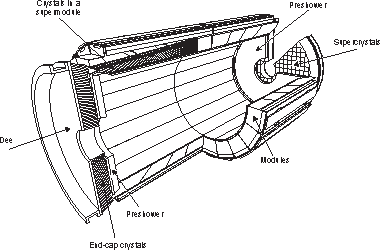
\includegraphics[width=\textwidth]{figures/cms_ecal_schematic.pdf}
  \end{minipage}
  \begin{minipage}[c]{.38\textwidth}
    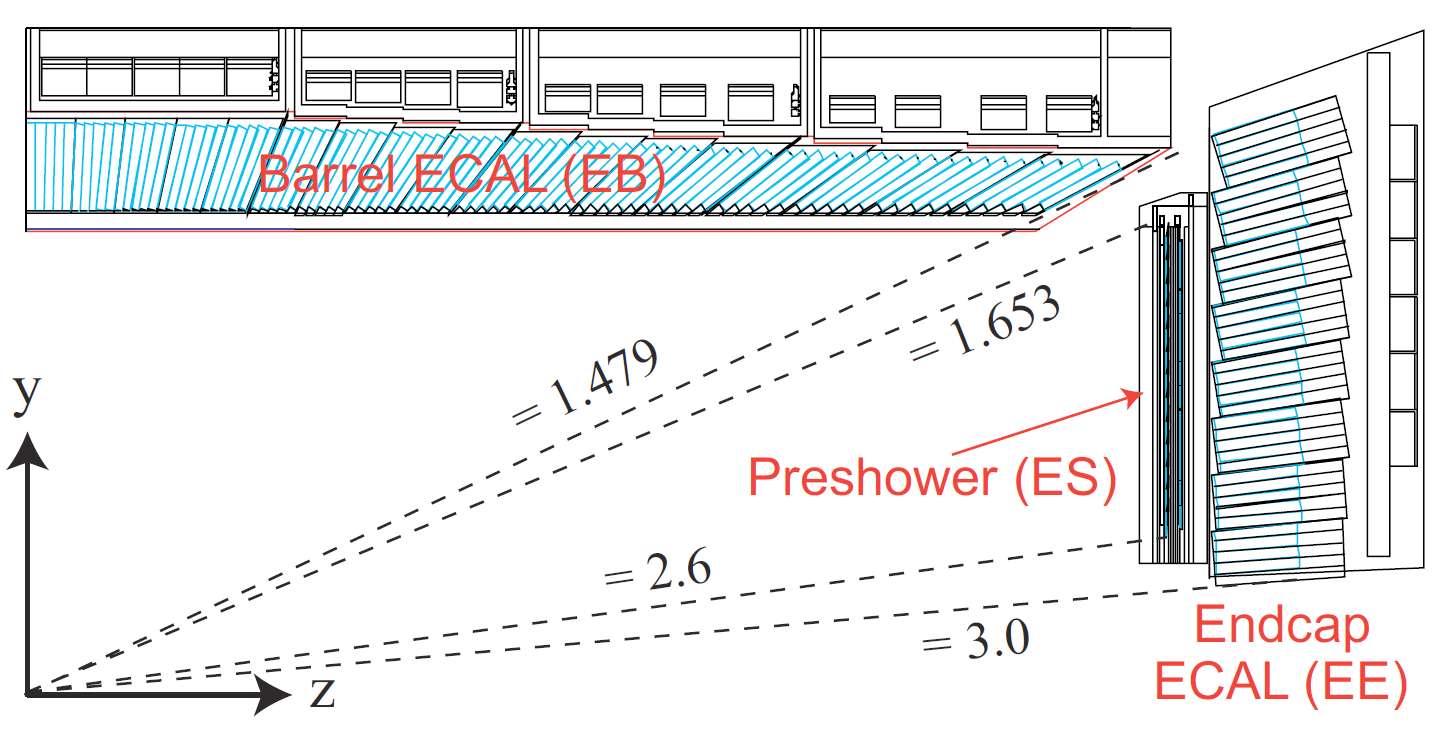
\includegraphics[width=\textwidth]{figures/cms_ecal_layout.png}
  \end{minipage}
  \caption[The CMS \gls{ECAL} schematic layout]%
  {The \gls{CMS} \gls{ECAL} schematic layout. The left is schematic showing arrangement of
    superclusters in barrel and endcap (with preshower layers). The right is \(y-z \)
    plane quarter view of \gls{ECAL} layout~\cite{image-cms-ecal-layout}.}%
  \label{fig:cms-ecal-schematic}
\end{figure}

The resolution of the \gls{ECAL} energy measurements can be described as,

\begin{equation}
  {\left( \frac{\sigma}{E} \right)}^2
  = {\left( \frac{S}{\sqrt{E}} \right)}^2
  + {\left( \frac{N}{E} \right)}^2
  + C^2
\end{equation}

where \(S \) is the stochastic term, \(N \) is related to the noise,
and C is a constant offset.

\begin{figure}[!ht]
  \centering
  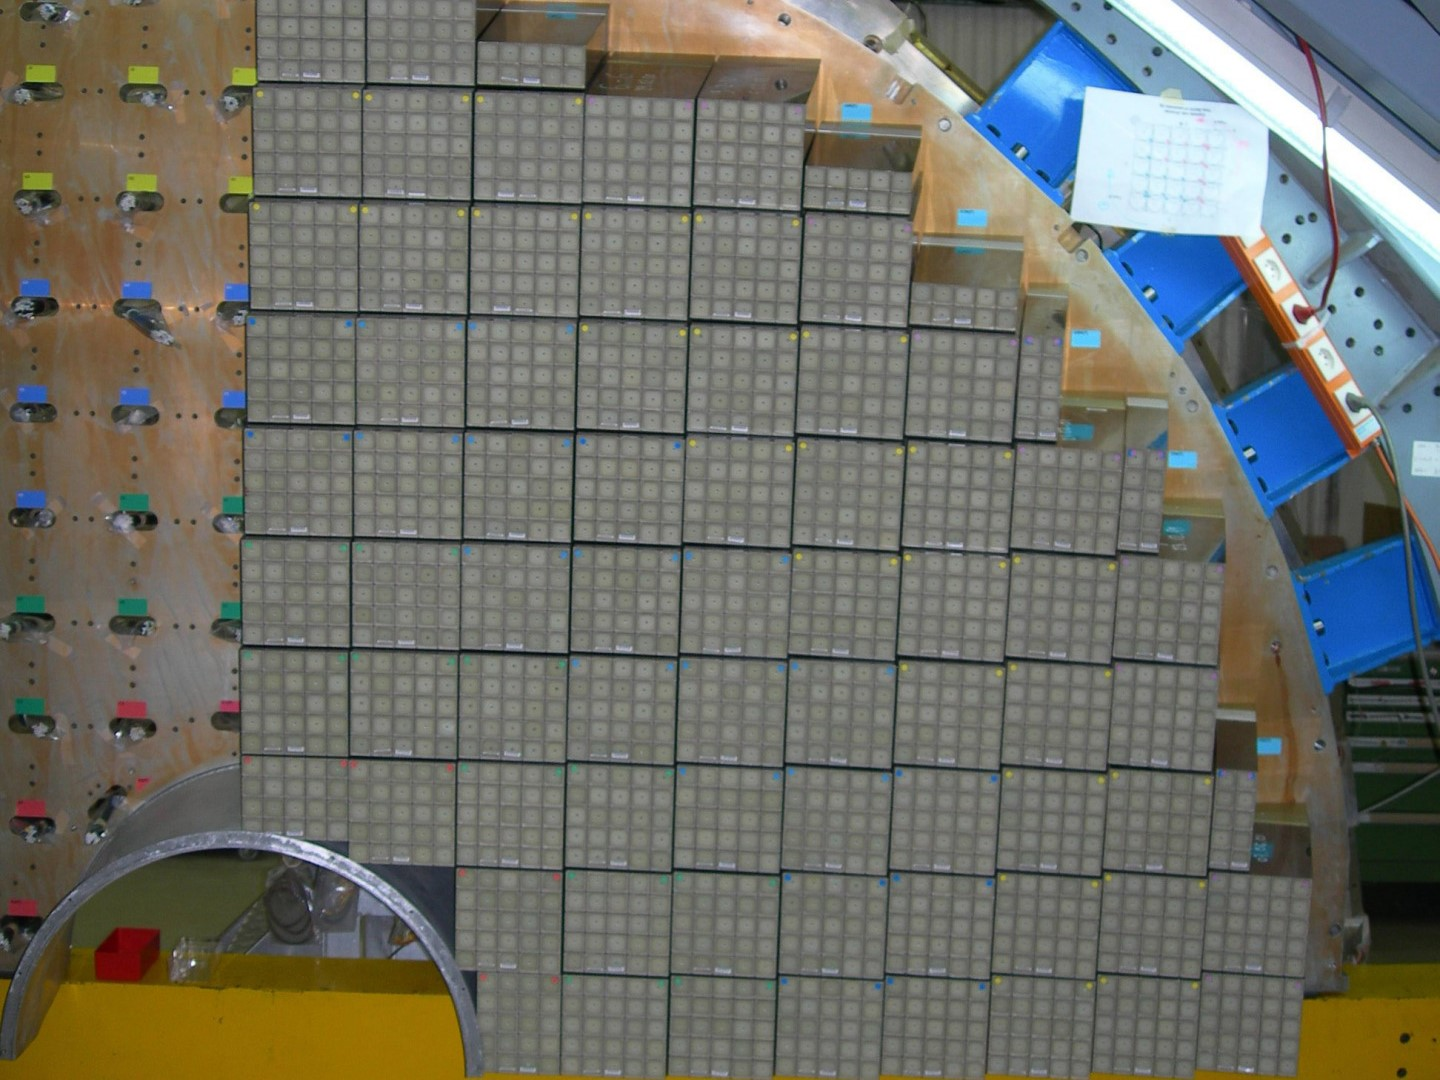
\includegraphics[width=0.60\textwidth]{figures/cms_ecal_ee_quadrant.jpg}
  \caption[The \gls{ECAL} endcap quadrant assembled view]%
  {The \gls{ECAL} endcap quadrant assembled view~\cite{image-cms-ecal-ee-quadrant}.}%
  \label{fig:cms-ecal-ee}
\end{figure}

\subsection{
  The Hadronic Calorimeter
}

\gls{HCAL} is last subdetector inside solenoid after
\gls{ECAL} and the first half of barrel \gls{HCAL} inserted is shown in
Figure~\ref{fig:cms-hcal-inserted}. Similar to \gls{ECAL} the purpose of \gls{HCAL}
is to shower hadrons, and measure their energy and position. \gls{HCAL} is made up of
towers pointing towards \gls{IP} and each tower is made up of sampling layers
with alternating layers of plastic scintillator and brass.
Brass acts as absorber in \gls{HCAL} and causes hadrons to shower, then from the light
output of scintillator receiving secondary shower particles gives the amount of
energy deposit in each layer. In phase 1 upgrade the \gls{HCAL} was upgraded
to give energy deposit as function of depths and the depth segmentation schematic is
show in Figure~\ref{fig:cms-hcal-depth} and the details of upgrade are in technical design
report~\cite{cms-hcal-upgrade}.

\begin{figure}[!ht]
  \centering
  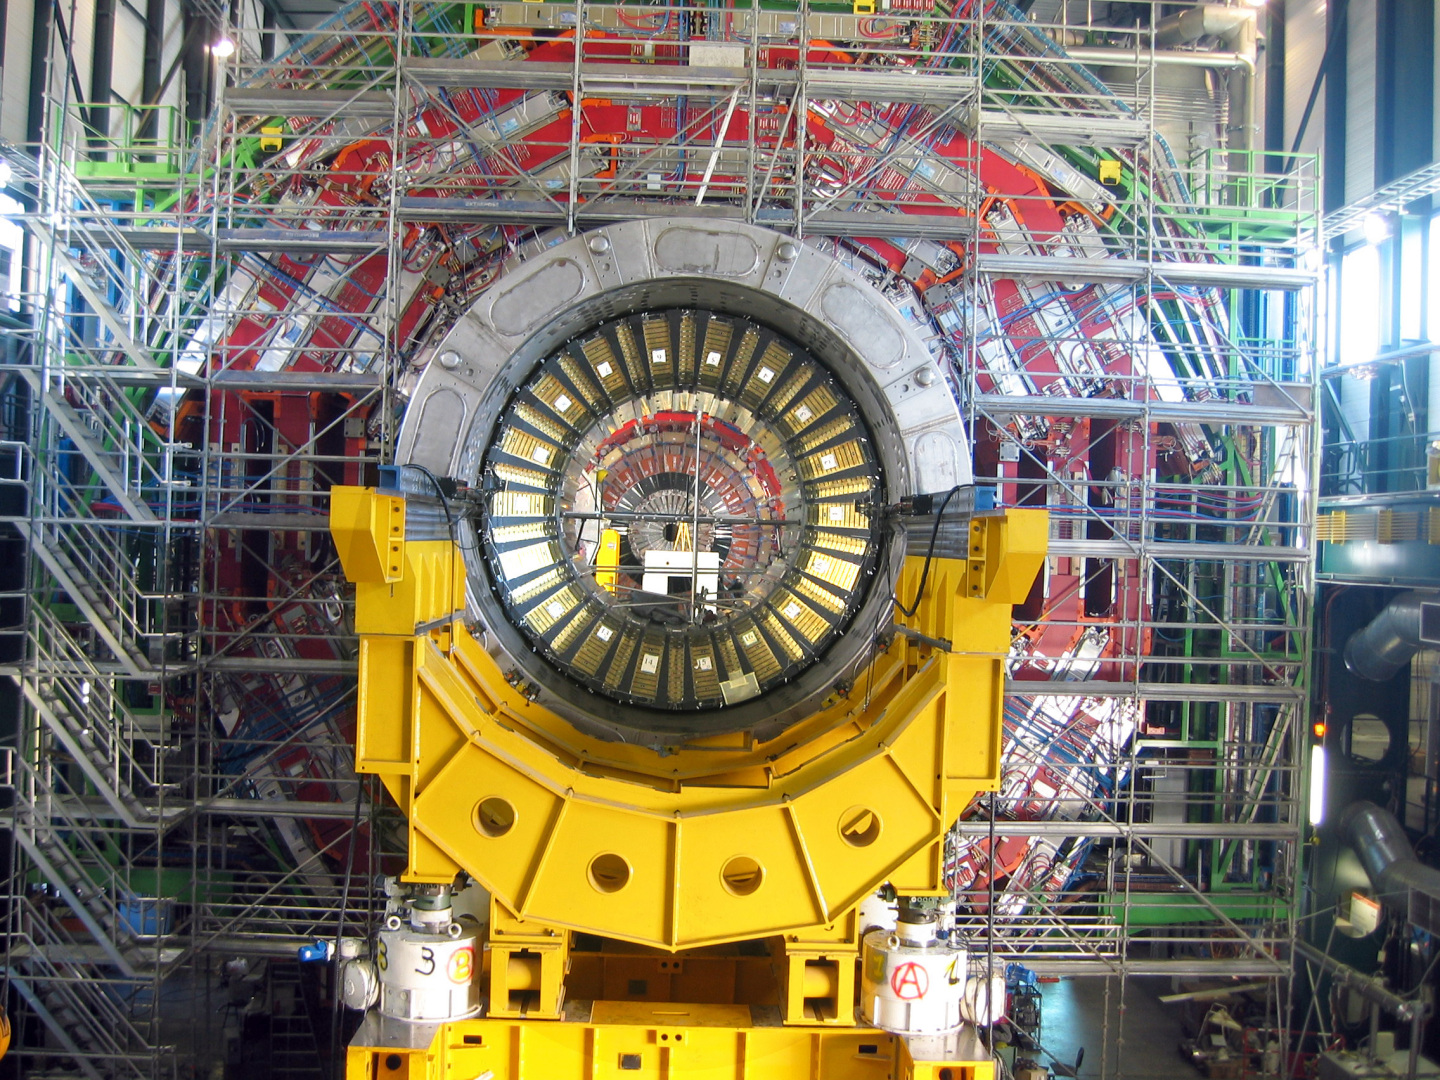
\includegraphics[width=\textwidth]{figures/cms_hcal_hb_inserted.jpg}
  \caption[The first half of the barrel \gls{HCAL} inserted into the
    superconducting solenoid (April 2006)]%
  {The first half of the barrel \gls{HCAL} inserted into the
    superconducting solenoid (April 2006)~\cite{image-cms-hcal-inserted}.}%
  \label{fig:cms-hcal-inserted}
\end{figure}

\gls{HCAL} consists barrel (HB) and two endcaps (HE) located inside solenoid.
These two subsystems combined cover region \( |\eta| = 3.0 \), which
is most of physics analysis done in \gls{CMS}.
There are two another subsystems of \gls{HCAL} outside solenoid,
a forward \gls{HCAL} (HF) and outer barrel \gls{HCAL} (HO).
HO was added to ensure there is no leak from the particles that
make past the solenoid. HF extends the coverage
to \(|\eta| = 5.0\) and is based Cherenkov radiation principle unlike
other subsystems of \gls{HCAL}, and it uses quartz fiber
as active material with steel absorbers.
HF is used most commonly used by heavy ion analysis.

\begin{figure}[!ht]
  \centering
  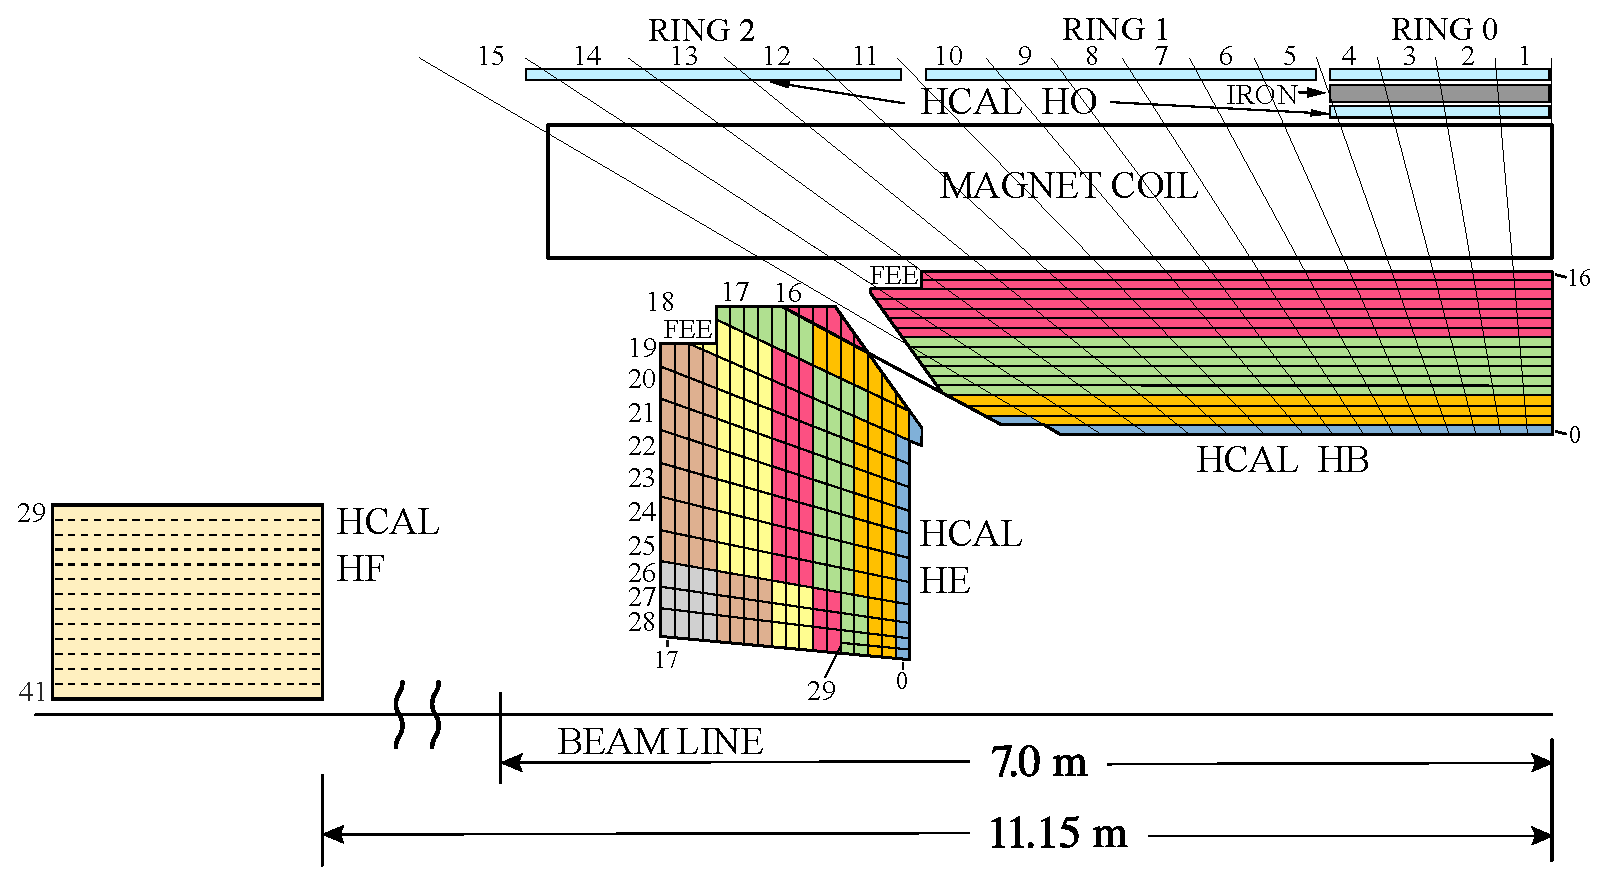
\includegraphics[width=\textwidth]{figures/cms_hcal_depth_seg.pdf}
  \caption[The \gls{HCAL} depth segmentation after phase 1 upgrade]%
  {The \gls{HCAL} depth segmentation after phase 1 upgrade~\cite{image-cms-hcal-depth}.}%
  \label{fig:cms-hcal-depth}
\end{figure}

\subsection{
  Muon Detector
}

The outermost subsystem in the \gls{CMS} detector is the muon detector.
Unlike electrons, muons are \glspl{MIP}, they do not lose much of their energy
while passing through tracker, calorimeter and solenoid.
Muon detector is build to identify, measure momentum and trigger the events
with muons. Like other subsystems, muon detector consists of barrel and endcap
detector and schematic layout is highlighted in Figure~\ref{fig:cms-muon-system}.

The muon detector consists of three subsystems \glspl{DT}, \glspl{CSC} and
\glspl{RPC}.

The \glspl{DT} are wire gas detectors filled with Argon and composed of
many tube cells of about 4\cm{}. Muon passing through these tubes
ionizes Argon and free electron is detected with wires as cathode.
Each DT is about 2 meters by 2.5 meters in size, and there are four layers
of the \glspl{DT} interleaved with iron yoke parallel to
the beam pipe in barrel region. The drift time is the order of about 380\nanoseconds.

\begin{figure}[!ht]
  \centering
  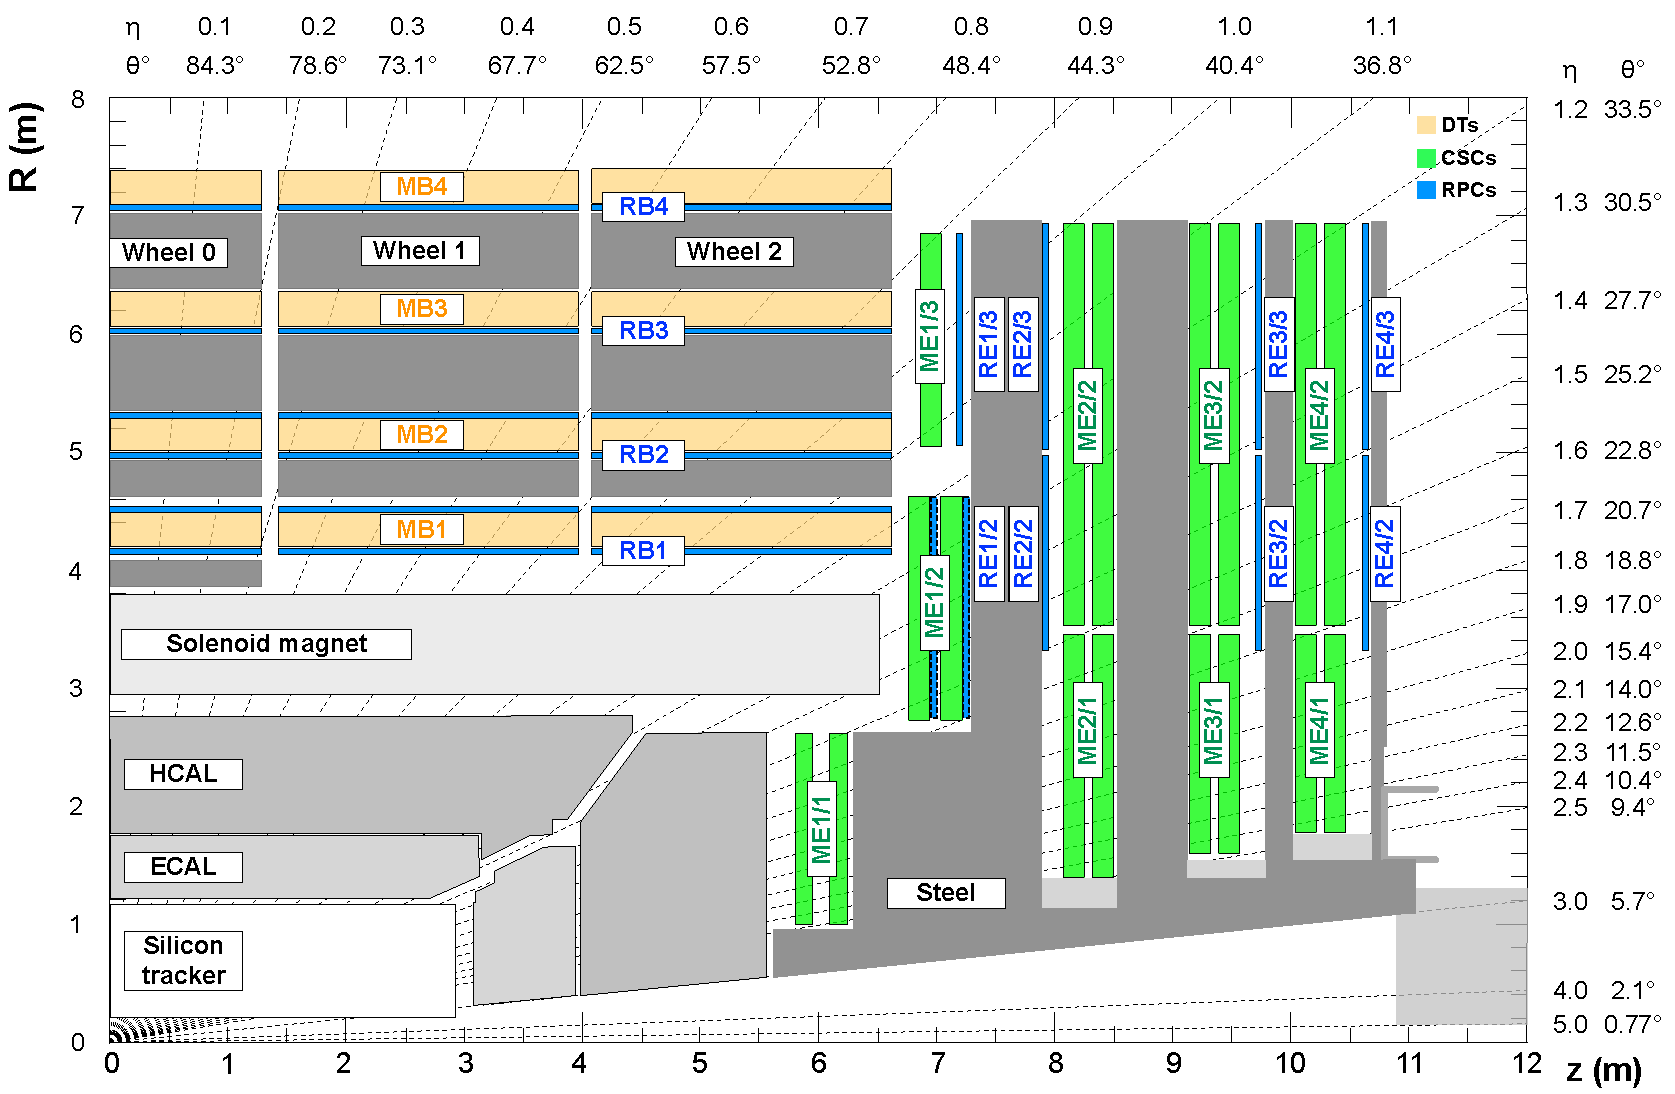
\includegraphics[width=0.9\textwidth]{figures/cms_muon_system.pdf}
  \caption[The quadrant view of CMS subdetectors layout, and
    the coverage of the muon detector \glspl{DT}, \glspl{CSC},
    and \glspl{RPC} highlighted]%
  {The quadrant view of CMS subdetectors layout, and
    the coverage of the muon detector \glspl{DT}, \glspl{CSC},
    and \glspl{RPC} highlighted~\cite{image-cms-muon-system}.}%
  \label{fig:cms-muon-system}
\end{figure}

The \glspl{CSC} are based on same principle as \glspl{DT},
and are made of multi-wire proportional chambers consisting of
6 anode planes interleaved with 7 cathode planes. They have time resolution
smaller than 5\nanoseconds. The \glspl{CSC} are used in endcap region,
where radiation hardness is required, and non uniform magnetic field does neutrinos
effects the the measurement.

The \glspl{RPC} are made up of two high resistive parallel
plates, with oppositely charged plates and gas volume between them.
When a charged particles passes through it and ionizes the gas, it creates
an avalanche and charge is collected by metallic readout strips.
\glspl{RPC} have poor position resolution but fast readout of the order of 1\nanoseconds,
which is fast compared to \glspl{DT}, this is the reason there are 1 or 2 \glspl{RPC}
attached to both \glspl{DT}, and \glspl{CSC}.

\subsection{
  Level 1 Trigger
}

Since proton-proton collisions happens every bunch crossing which is
25\nanoseconds{} apart, which is equivalent to 40\,\text{MHz}\xspace collisions rate.
At this collisions rate, the data storage required will be enormous
and \gls{CMS} can only record up to 1000 events per second. Since most of events
does not contain interesting physics events, they can be thrown away.
To do this \gls{CMS} has two tier trigger system \gls{L1T}, and \gls{HLT}.

The \gls{L1T} is the foremost electronic processing system through
which event information is processed before it is passed to
second trigger system \gls{HLT}.
The \gls{L1T} is designed to make fast decisions in about 3.8\mus,
and only uses \gls{ECAL}, \gls{HCAL} and muon system to make decision.
\gls{L1T} cut downs the data rate from 40\,\text{MHz}\xspace to
100\,\text{kHz}\xspace. The \gls{L1T} electronics is placed next to
the detector in underground cavern for fast transfer of data.

The \gls{HLT} further reduces the data rate from 100\,\text{kHz}\xspace to
about 1\,\text{kHz}\xspace using a computer farm with nearly 26000 cores.
\gls{HLT} uses all the available information from the event to make
decision in about 300m\seconds. \gls{HLT} is modular by design
to allow the use of information from different systems to construct
multiple paths called \gls{HLT} paths, for example the single muon \gls{HLT}
path will save event with at least one muon passing the selection criteria
set in \gls{HLT} path. Events passing at least on \gls{HLT} path are
save for offline physics analysis.

\section{
  High Granularity Calorimeter Upgrade
 }

About \gls{HGCAL} Upgrade

\subsection{
  Technical Design
}

\begin{figure}[!ht]
  \centering
  \begin{minipage}[c]{0.49\textwidth}
    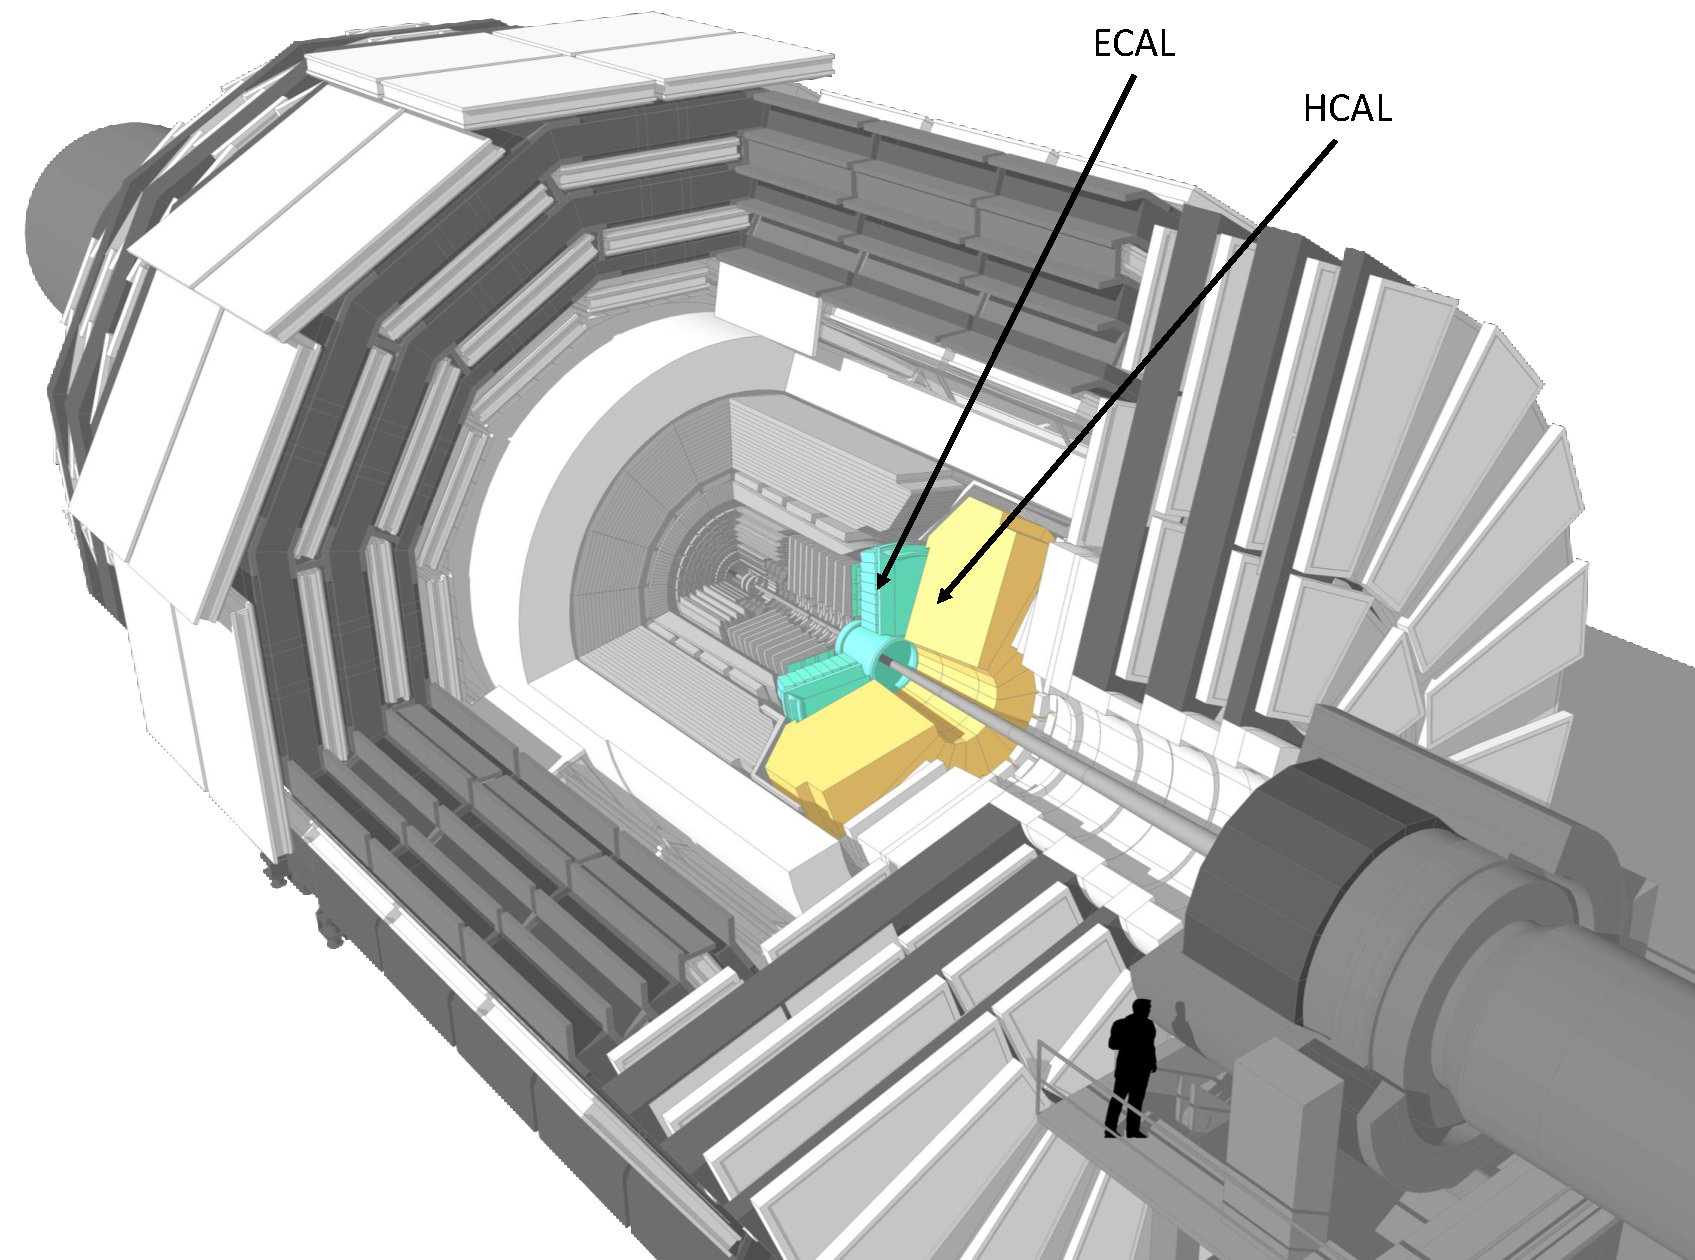
\includegraphics[width=\textwidth]{figures/hgcal/hgcal_place.pdf}
  \end{minipage}
  \begin{minipage}[c]{0.49\textwidth}
    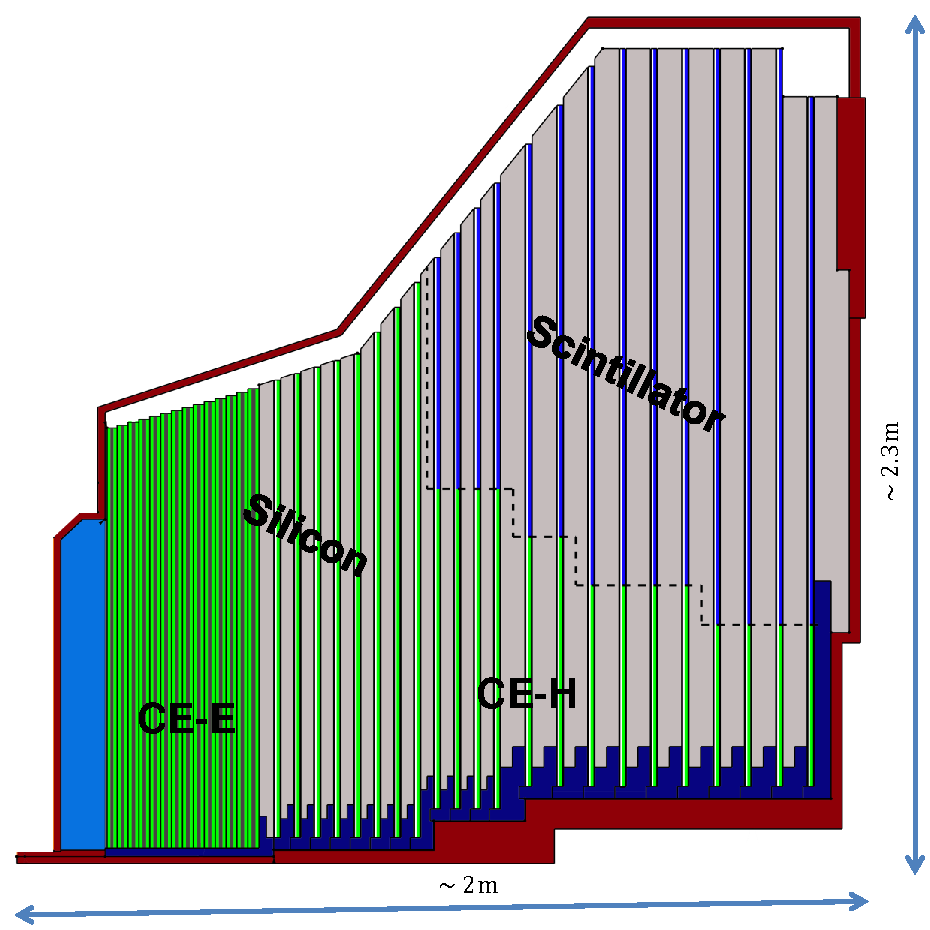
\includegraphics[width=0.9\textwidth]{figures/hgcal/hgcal_quadrant.pdf}
  \end{minipage}
  \caption[Overview of CE]%
  {Overview of CE~\cite{image-cms-hgcal-quadrant-layout,image-cms-hgcal-place}}%
  \label{fig:cms-hgcal-quadrant-layout}
\end{figure}

\subsection{
  Scintillator Tiles
}

%\begin{figure}[!ht]
%  \centering
%  \includegraphics[width=\textwidth]{figures/hgcal/}
%  \caption[SiPM]{SiPM}%
%  \label{fig:hgcal-sipm}
%\end{figure}

\subsection{
  End of Life Scenario
}

\begin{figure}[!ht]
  \centering
  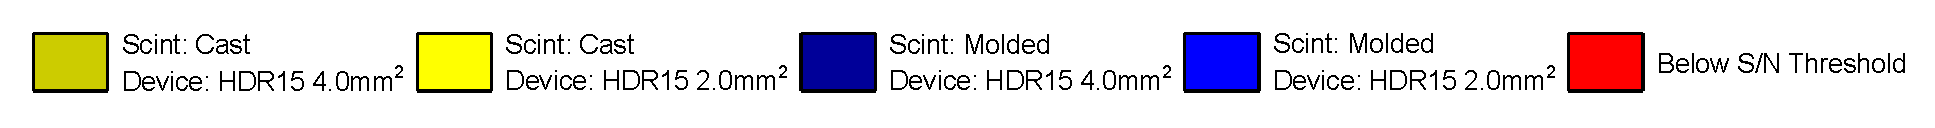
\includegraphics[width=\textwidth]{figures/hgcal/scenes_legend.pdf}
  \begin{minipage}[c]{0.49\textwidth}
    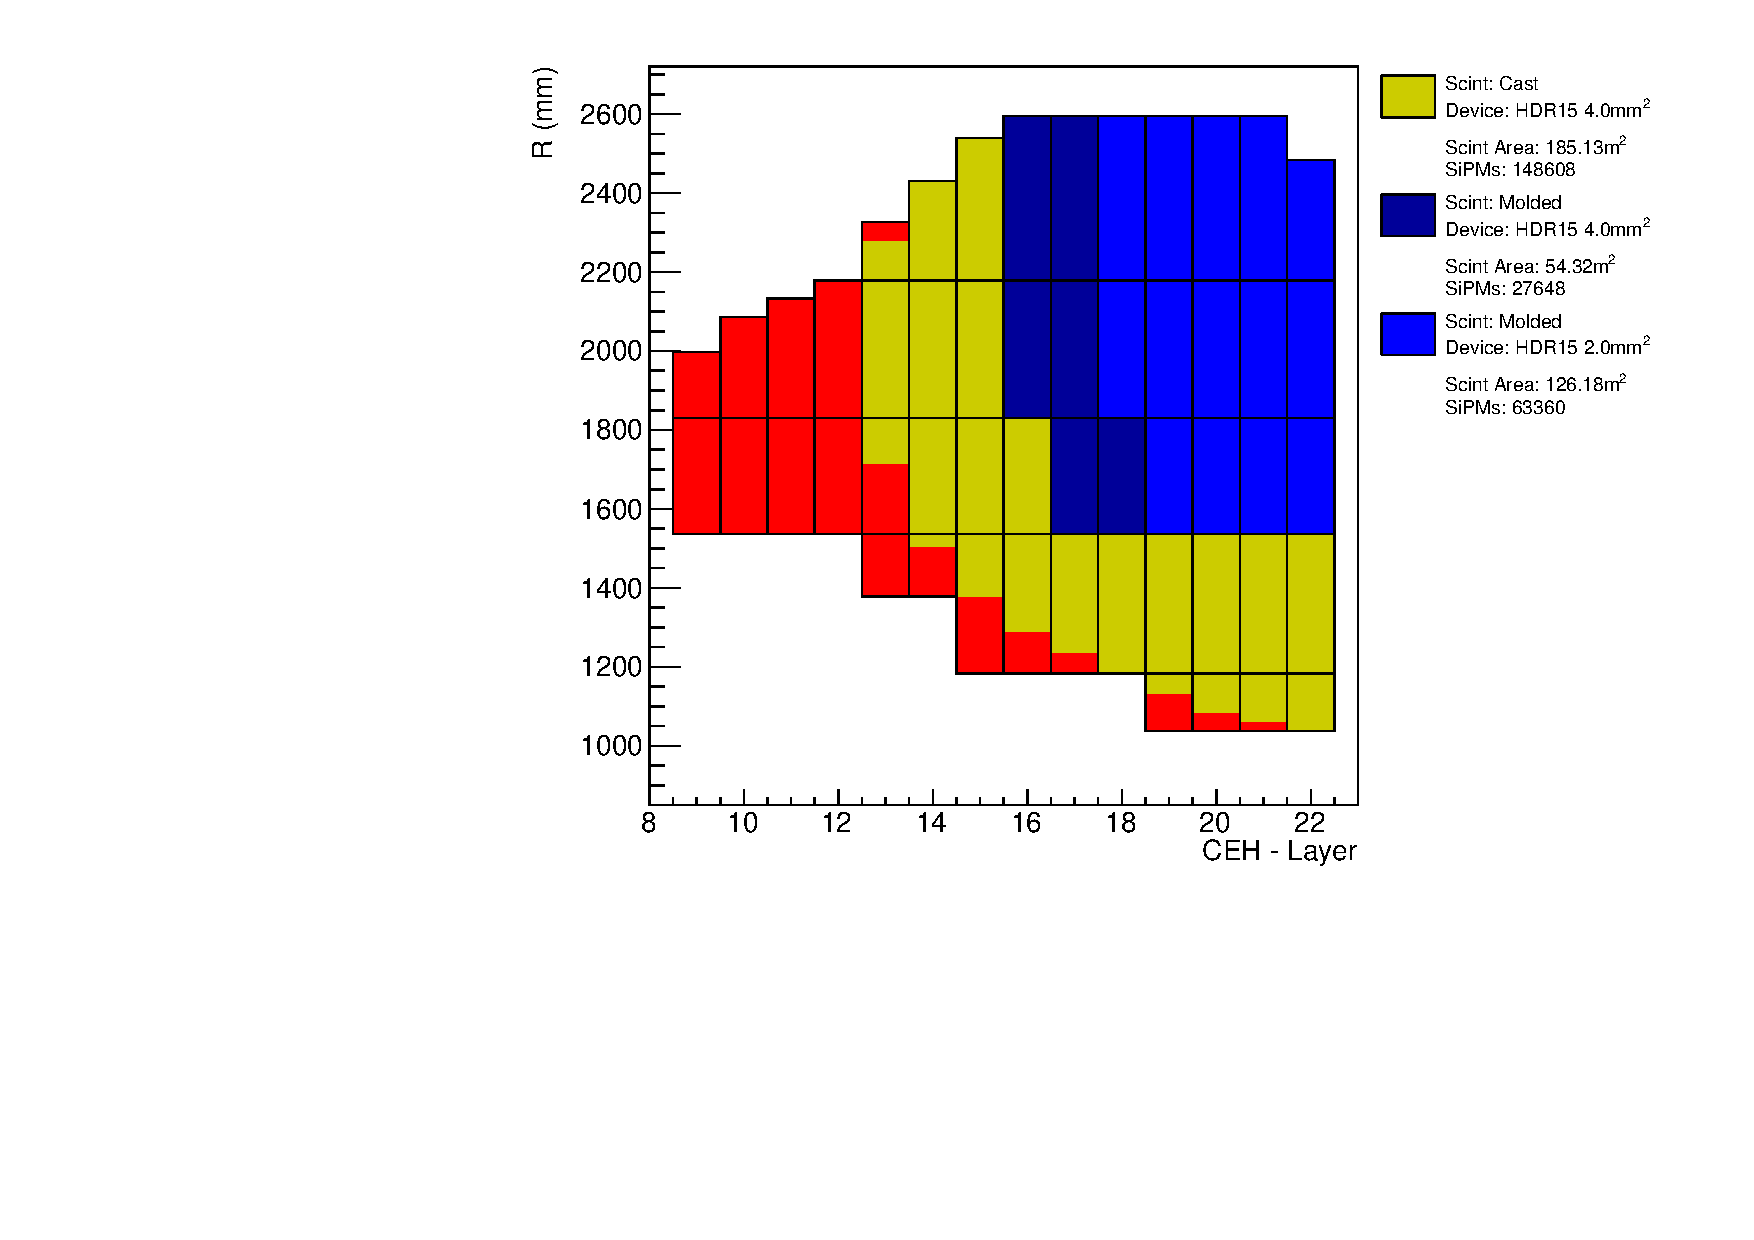
\includegraphics[trim={0 0 165pt 0},clip,width=\textwidth]{figures/hgcal/sceneA_jan20_2.pdf}
  \end{minipage}
  \begin{minipage}[c]{0.49\textwidth}
    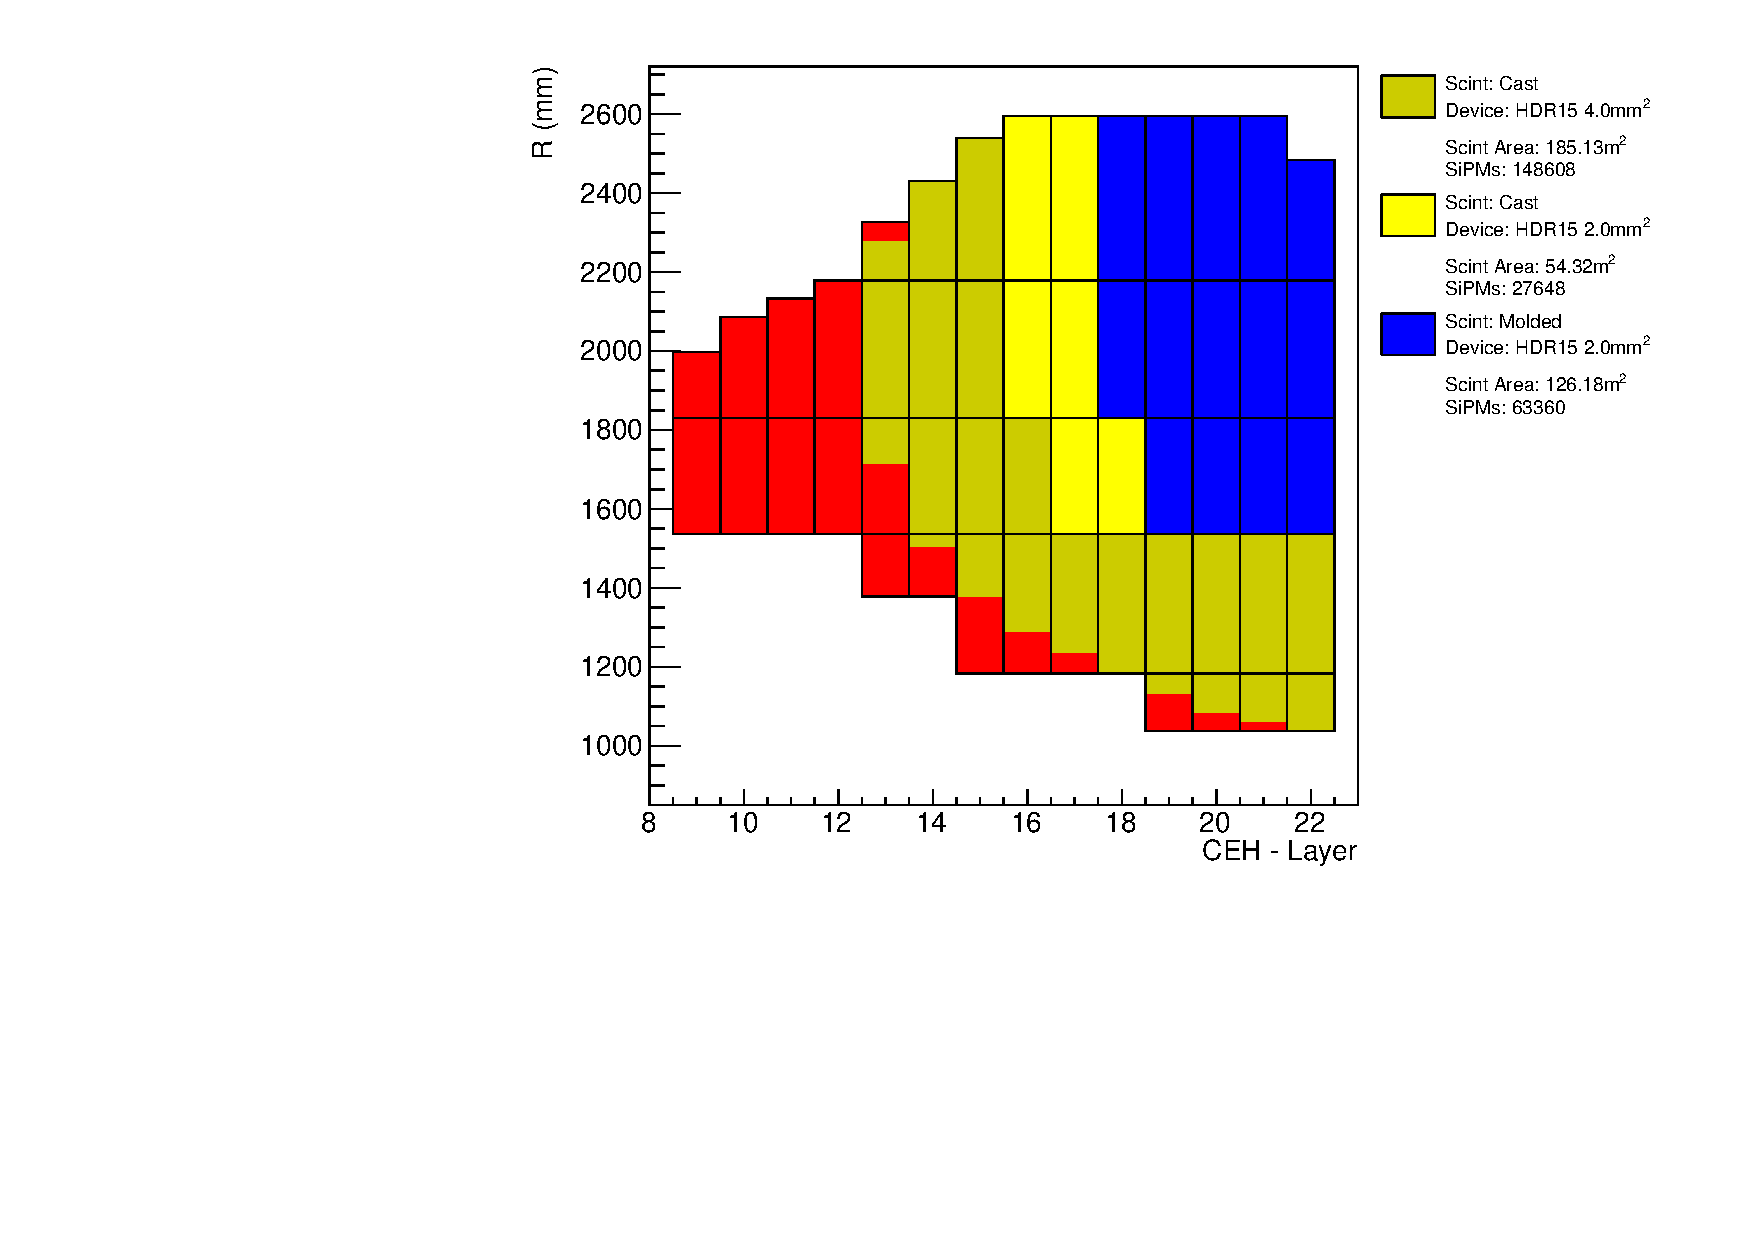
\includegraphics[trim={0 0 165pt 0},clip,width=\textwidth]{figures/hgcal/sceneB_jan20_2.pdf}
  \end{minipage}
  \caption[\gls{HGCAL} scenarios]{\gls{HGCAL} scenarios}%
  \label{fig:hgcal-scenes-fnal-jan20}
\end{figure}

\begin{table}[!ht]
  \centering
  \caption{\gls{HGCAL} scenarios comparison}
  \begin{tabular}{p{1.5in}cll}%
    \toprule
                                                   &                    & Scene A                & Scene B                \\
    \midrule
    \multirow{3}{=}{Cast Scintillator}             & Cell Count         & 148, 608               & 176, 256               \\
                                                   & Total Area         & 185.13 \(\text{m}^2 \) & 239.45 \(\text{m}^2 \) \\
                                                   & Percentage         & 50.6 \%                & 65.5 \%                \\
    \cmidrule(lr){2-4}
    \multirow{3}{=}{Injection Molded Scintillator} & Cell Count         & 91, 008                & 63, 360                \\
                                                   & Total Area         & 180.5 \(\text{m}^2 \)  & 126.18 \(\text{m}^2 \) \\
                                                   & Percentage         & 49.4 \%                & 34.5 \%                \\
    \cmidrule(lr){2-4}
    \multirow{2}{=}{SiPMs Count}                   & 2 \(\text{mm}^2 \) & 63, 360                & 91, 008                \\
                                                   & 4 \(\text{mm}^2 \) & 100, 224               & 148, 608               \\
    \bottomrule
  \end{tabular}
\end{table}